\chapter{Related Work}\label{ch3}

% GOAL:
% rearrange statements to properly cite references
% add background section which includes: common patterns for IoT/Web app: RESTful, Pub/Sub, Observer; an overview to the Erlang language (data type, pattern matching, function and module, process, message passing, concept of OTP)

\section{Background} \label{background}

\subsection{IoT and Fog Computing} 

Recently, researchers have shown an increased interest in the Internet of Things (IoT). The IoT aims at providing an intelligent environment where ubiquitous goods in the the physical world can be connected to the Internet through unique addressing schemes so that they can interact with each other and cooperate with their neighbours to reach common goals without human involvement \autocite{Atzori20102787}.  It is enabled by a variety of technologies including Radio-Frequency Identification (RFID), smart sensors and actuators, mobile computing and Internet protocols \autocite{7123563}. Potential application areas in IoT range from transportation and logistics, healthcare, social networking, smart environment (home, office, plant), industrial automation, to emergency response to disasters and more other areas \autocite{Atzori20102787, 7123563}. The US National Intelligence Council (NIC) considers the IoT as one of the six ``Disruptive Civil Technologies” that will have an impact on US National Power and indicates that ``by 2025 Internet nodes may reside in everyday things -- food packages, furniture, paper documents, and more'' \autocite{strategic2008disruptive}. It is estimated that 28.1 billion IoT devices will be connected which brings a 7.1 trillion dollars worldwide market by the end of 2020 \autocite{lund2014worldwide}.

The vision of IoT has foreseen many common challenges, among which, scalability and reliability are more critical than ever \autocite{Atzori20102787, 7123563, 8058399}. Over the past decade, the industry has seen a trend of moving computing and storage resource behaviourinto the Cloud. It is straightforward to integrate the IoT with the Cloud to address the scalability and reliability issue. However, the emerging IoT introduces many new challenges that can not be adequately addressed by today's Cloud Computing models alone. These challenges \autocite{7498684, 7033259} include but are not limited to, stringent latency requirements under certain environment (such as industrial control systems), inflexibility of the Cloud supporting rapid mobility patterns, network bandwidth limitation due to rapid growing number of connected things, difficulty for resource-constrained devices to interact with the Cloud using complex protocols, applications which require uninterrupted services but with intermittent connectivity to the Cloud, and security concerns caused by the combinations of one or more issues mentioned above.

\begin{figure}[!htbp]
\centering
\includegraphics[scale = 0.55]{Fog_computing.png}
\caption[The role of the Cloud and Fog play in the delivery of IoT services]{The role of the Cloud and Fog play in the delivery of IoT services. \autocite{7123563}} 
\label{fig:Fog_computing}
\end{figure}

In order to fill the technology gaps in supporting the IoT, a new architecture - Fog Computing - was first introduced. Fog is an architecture where computation, networking and storage are arranged closer to end devices instead of inside Cloud data centres \autocite{Bonomi:2012:FCR:2342509.2342513}. Fog consists of heterogeneous, potentially wide-spread and geographically distributed networks of nodes, where a node can be any smart edge device or system that acts as a local intelligence for all related sensors and actuators. A Fog in each location can be as small as a single node or as large as required to meet customer demands and many small Fog nodes may constitute a large Fog system \autocite{7498684}. 

The primary idea behind Fog Computing is to put the force of analyzing and processing data to applications hosted by devices within the network instead of to a centralized Cloud \autocite{7033259}. As a result, it enables IoT applications which require low-latency, location-awareness, real-time interactions and analytics and mobility support. Fog also enhances the scalability and resilience of IoT applications by its nature \autocite{7123563}. Various services and computing tasks can run on a Fog node, depending on how much resource a node owns and application-specific requirements. Applications could on the one hand let local Fog carry out resource-intensive tasks (M2M interaction, data collection and processing, actuator control, etc.) on behalf of resource-constrained devices when such tasks cannot be moved to Cloud due to latency constraints or any other reasons, on the other hand expect the preprocessed data to be consumed by higher tiers, which can be other Fog or the global Cloud, for long-term analysis and storage \autocite{7498684}. \autoref{fig:Fog_computing} illustrates the roles that the Cloud data centres and the Fog play to deliver IoT services to end-users. 

Fog Computing has the potential to increase the overall performance of IoT applications. Scenarios where Fog could help include low-latency applications such as gaming and video conferencing, geo-distributed applications such as pipeline monitoring and wireless sensor networks, fast mobile applications such as connected vehicle and connected rail, and large-scale distributed control systems such as smart grid and smart traffic
light systems \autocite{bonomi2014fog}. A real-world success of Fog has been discussed in \autocite{7498684}, where Barcelona utilized Fog as a uniform platform for all services in their smart city management applications and reduced overall system costs.

Fog Computing provides a new application scenario for this work apart from the Cloud. Scalability and reliability are still required on a Fog node especially when complex tasks and services are deployed. The Fog node is highly possible a less-constrained embedded device such as the Raspberry Pi \autocite{raspberry_pi}, which has more resources than ordinary sensors and actuators yet is much less powerful than the Cloud. Moreover, since the Constrained Application Protocol (CoAP) is a standard machine-to-machine (M2M) protocol, it surely has its use space under a Fog environment. It is therefore considered the combination is not only a valid use case in terms of Fog Computing, but also falls within the scope of this thesis. 

\subsection{Common Patterns of IoT Applications}

Some of the architectural patterns that are common in other information systems can be applied to the design of IoT applications as well. This section introduces three most widely used ones: REST, publish/subscribe and observer pattern.

\subsubsection{REST}

The Representational State Transfer (REST) was first defined by \textcite{fielding2000architectural} in his doctoral dissertation in 2000. It is an architectural style that defines constraints for creating Web services, and its principles were used in designing the HTTP 1.1 \autocite{http1.1} and Uniform Resource Identifiers (URI) \autocite{uri_rfc} standards. Web services that follow the REST style are claimed as RESTful, which provide interoperability to a majority of computers connected to the Internet nowadays. Though REST is not tied to any particular technology, HTTP, which has four basic operations (HTTP verbs): GET, POST, PUT and DELETE, is commonly used as its pattern matches REST well. In general, REST defines the behaviour of a well-designed Web service, which should consist of a network of Web resources that the user could go through via corresponding links and applying operations such as the HTTP verbs to0. The operations trigger state transitions of the resource and as a result, the next resource is transferred to the user. 

Some of the important characteristics of REST are:

\begin{itemize}
\item REST relies on the client-server hence request-response model.
\item REST identifies resources using URIs.
\item REST uses stateless operations upon resources.
\item REST separates resources from their representations.
\end{itemize}

Modern Web applications extensively use REST since its semantics naturally allows for caching, proxying and redirecting requests/responses between Web resources distributed over loosely coupled Internet endpoints, resulting in a highly flexible, scalable, reliable and interoperable architecture.

\subsubsection{Publish/Subscribe}

Publish/subscribe is a messaging pattern that provides loosely coupled interactions. The receivers of messages, called subscribers, could specify their interest in messages of certain patterns and are subsequently notified asynchronously of any message that is produced by the senders of messages, called publishers when the message matches the registered interest \autocite{6918928}. Since subscribers only receive a subset of all published messages, publish/subscribe systems differ in the way of selecting the messages of interest and can be primarily classified to following types:  topic-based, content-based and type-based \autocite{Eugster:2003:MFP:857076.857078}. In a topic-based system, messages are classified by topics and subscribers only receive messages published to the topics that they subscribe. In a content-based system, messages are delivered to subscribers if they match certain constraints the subscribers to define over the properties of the message and are not pre-classified. In a type-based system, messages are also filtered based on the type or class, which can be defined, for example, using object-oriented languages.

Publish/subscribe pattern has the following advantages:

\begin{itemize}
\item Space decoupling: Publisher and subscriber do not need to know each other.
\item Time decoupling: Publisher and subscriber do not need to be active at the same time.
\item Synchronization decoupling: Publisher and subscriber do not block each other when publishing and receiving messages.
\end{itemize}

A publish/subscribe service can be implemented with a centralized broker, which stores and manages subscriptions. It can also be realized in a distributed manner, where the management work is implemented both in publishers and subscribers. The former brings stronger reliability while the latter is more scalable \autocite{Eugster:2003:MFP:857076.857078}.

\subsubsection{Observer Pattern}

Observer pattern \autocite{gamma1995design} is a term used more commonly in object-oriented software designs. 

It defines the relationship of a ``subject'' and one or more ``observers'', where a subject has the state of interest and maintains a list of all dependencies, called observers, who register themselves at the subject and are interested in being notified whenever the state undergoes a change. The observer pattern itself shares similarities with publish/subscribe pattern. The main difference is that in observer pattern the subject is aware of the observers and maintains states about them, while in publish/subscribe pattern both parties of the interaction are decoupled.

In summary, all the above patterns can be useful when designing IoT applications. the REST architectural style essentially brings what makes the current Web robust to the IoT field, so that an IoT application exposing as a RESTful service can easily reuse existing Web capabilities. The publish/subscribe pattern is extremely useful when the producer and consumer of IoT services are not synchronous by their nature. The observer pattern, being a variation of the publish/subscribe pattern, is used by CoAP to realize resource state observation, which does not fit naturally with the stateless REST style.

\subsection{A Brief Introduction to Erlang/OTP}

% outline:
% data type including atom
% function and module
% pattern match 
% otp

This section contains a short summary of concepts of the Erlang language that are important to this work. 

Erlang is a single assignment, dynamically typed functional language. Single assignment means that a variable gets bound to a particular value and can not be reassigned to a different value. In Erlang, a variable starts with a capital letter. Some of the basic data types of Erlang are:

\begin{itemize}
\item Term: A term is of any data type.
\item Number: A number can an integer, e.g. \verb|5|, or a float, e.g. \verb|1.5|.
\item Atom: An atom is a literal constant with a name. It is to be enclosed in single quotes if it does not begin with a lower-case letter or if it contains other characters than alphanumeric characters, underscores, or at signs. e.g. \verb|red|, \verb|a_long_name|. Note there is no boolean type and \verb|true|, \verb|false| are of atom type.
\item Tuple: A tuple is a compound data type with a fixed number of terms. e.g. \verb|{john, {july, 24}}|.
\item List: A list of a compound data type with a variable number of terms. e.g. \verb|[a,2, {c, 4}]|.
\item String: A string is enclosed in double quotes, and is actually a list of integers where each integer represents a Unicode codepoint. e.g. \verb|"Hello"|.
\item Bit string and binary: A bit string is used to store an area of untyped memory. Bit strings that consist of a number of bits that are evenly divisible by eight, are called binaries. e.g. \verb|<<"ABC">>|, \verb|<<1:1,0:1>>|.
\item Record: A record is a data structure for storing a fixed number of elements and is to be transferred to tuple during compilation. Example of defining a record: \verb|-record(person, {name, age})|. Example of initializing a record: 
\verb|#person{name=Name, age=Age}|.
\item Map: A map is a compound data type with a variable number of key-value associations. Key can be any valid Erlang term. e.g. \verb|#{name=>adam, age=>24, date=>{july, 29}}|
\item Pid: A pid is a unique process identifier. e.g. \verb|<0.100.0>|.
\item Reference: A reference is a globally unique Erlang term created using the built-in functions.
\end{itemize}

\begin{listing}[!htbp]
\centering
\begin{minted}
[bgcolor=bg,
frame=lines,
framesep=2mm,
baselinestretch=1.2,
fontsize=\footnotesize,
linenos=true]
{erlang}
-module(math).
-export([fac/1]).

fac(N) when N > 0 -> N * fac(N-1); 
fac(0) -> 1.
\end{minted}
\caption{Erlang factorial example}
\label{lst:erlang_fac_example}
\end{listing}

\autoref{lst:erlang_fac_example} shows a sequential program which calculates the factorial of \verb|N|. It starts with a module definition and a list of exported functions. Erlang programs are organized through files called modules each containing a sequence of function declarations. Each function declaration is a sequence of function clauses separated by semicolons, and terminated by a period \verb|(.)|. A function clause consists of a clause head and a clause body, separated by \verb|->|, and an optional guard sequence beginning with the keyword \verb|when|. A clause head consists of the function name and an argument list. The function name is an atom. Each argument is a pattern. The number of arguments N is the arity of the function. A function is uniquely defined by the module name, function name, and arity. A clause body consists of a sequence of expressions separated by a comma \verb|(,)|. A function named \verb|f| in the module \verb|m| and with arity \verb|N| is often denoted as \verb|m:f/N|, while an internal function can be referred to without specifying the module name. The example defines a \verb|math| module which exports a function named \verb|fac| that has one argument. The \verb|fac/1| function consists of two clauses. The first clause is a pattern that matches \verb|N>0| and executes recursively until hitting the base case, that is, \verb|fac(0)|. When another pattern occurs, the function clauses are scanned sequentially until one pattern matches otherwise the evaluation fails. 

\begin{listing}[!htbp]
\centering
\begin{minted}
[bgcolor=bg,
frame=lines,
framesep=2mm,
baselinestretch=1.2,
fontsize=\footnotesize,
linenos=true]
{erlang}
-module(counter).
-export([start/0, stop/1, add_number/2, get_number/1]).

start() -> 
    spawn(fun() -> loop(0) end).
    
add_number(Pid, M) ->
    Pid ! {add_number, M},
    ok.

get_number(Pid) ->
    Pid ! {get_number, self()},
    receive
	{counter, N} -> N
    end.
    
stop(Pid) -> 
    Pid ! stop,
    ok.
    
loop(N) ->
    receive
        {add_number, M} -> loop(N+M);
        {get_number, From} -> From ! {counter, N}, loop(N);
        stop -> ok
    end.

\end{minted}
\caption{Erlang messaging example}
\label{lst:erlang_message_example}
\end{listing}

\autoref{lst:erlang_message_example} shows a concurrent program where an Erlang process can be spawned which holds a counter while other processes can interact with it. By calling \verb|counter:start/0| a process is created which executes the \verb|loop/1| function, and the process identifier (PID) is returned. \verb|counter:add_number/1| accepts the Pid and a number \verb|M| as the argument, then sends a message \verb|{add_number, M}| to the counter process using the send operator \verb|!|. The counter process uses \verb|receive ... end.| syntax to pattern match received messages. If a message matches the corresponding clause is evaluated. If no clause matches the message will be left in the message box of the process. In the example, the above function call will make the counter process add the number \verb|M| together with the number it gets as its initial state, \verb|N|, and use the result as the new state for the next recursion loop. Similarly, \verb|counter:get_number/1| will trigger the counter process send back its state to the caller and \verb|counter:stop/1| will cause the counter process to exit the loop and hence terminate itself.

Real world Erlang applications seldom use plain Erlang extensively. Instead, the Open Telecom Platform (OTP) is preferred. It is a set of libraries and procedures for building scalable and fault-tolerant applications. The core concept of OTP is OTP behaviour. A behaviour encapsulates common behavioural patterns. It is driven by a parameterized callback module. In a word, the behaviour solves the nonfunctional parts of the problem, while the callback solves the functional parts. Most commonly used OTP behaviours include but are not limited to \verb|gen_server| which provides generic client-server abstraction, \verb|gen_statem| which provides a skeleton for the finite state machine, the \verb|supervisor| that describes the supervision architecture, etc. It is also possible to create user-defined behaviour. More details about behaviours used in this work can be found in \autoref{implementation}.

\section{Application Layer Protocols for IoT} \label{IoT_protocols}

Because of the fact that the IoT consists of a considerable amount of devices with vastly different capabilities, standards are in need to support interoperability between newer applications and services with existing hosts and IoT nodes \cite{cirani2015mjcoap}.  Among the many standards introduced facilitating interoperability, the Internet Protocol (IP) and application layer protocols are of the most importance, since the former enables devices to be part of the current Internet and the latter directly drives the development of different IoT services.

In general, current IoT application protocols can be divided into 3 types: message-oriented, data-oriented, and resource-oriented \autocite{7396558}. Representative protocols of the 3 types are Message Queue Telemetry Transport (MQTT) \autocite{mqtt_protocol}, the Data Distribution Service for real-time systems (DDS) \autocite{dds} and the Constrained Application Protocol (CoAP) \autocite{coap_protocol}. In this section, these protocols are discussed and compared in terms of their architecture and use cases. Reason for choosing CoAP as the protocol used in this work is also stated. 

\subsection{Message-oriented:  Message Queue Telemetry Transport (MQTT)}

Message Queue Telemetry Transport (MQTT) \autocite{mqtt_protocol} is a messaging protocol first introduced by IBM in 1999 and was later standardized by OASIS in 2013. It relies on a topic-based publish-subscribe architecture with a central message-broker that links the publishers and subscribers, as shown in \autoref{fig:mqtt}. It inherits advantages of publish/subscribe pattern, that is, decoupling of time, space and synchronization of both message producers and consumers. 

\begin{figure}[!htbp]
\centering
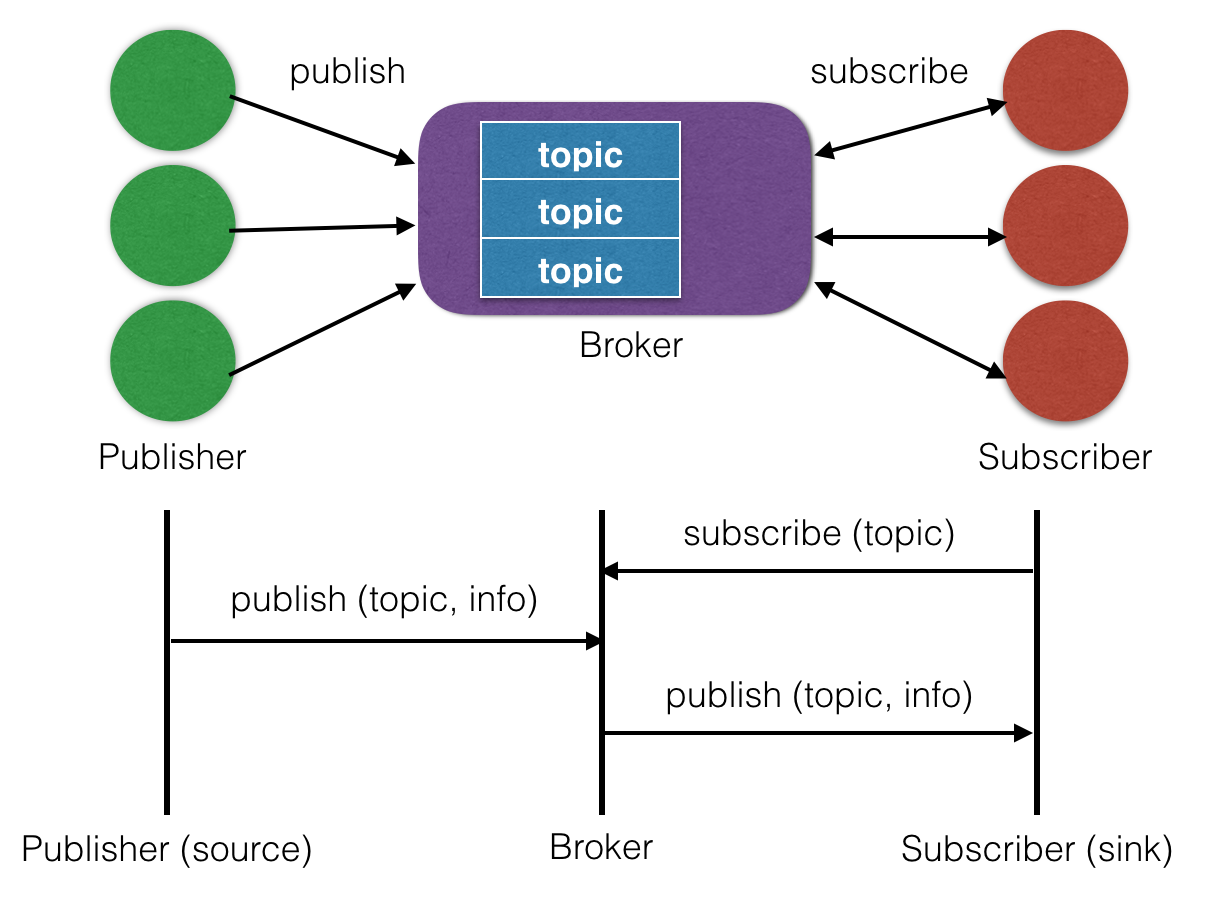
\includegraphics[scale = 0.55]{mqtt.png}
\caption{The architecture of MQTT and its publish/subscribe process}
\label{fig:mqtt}
\end{figure}

A typical workflow includes an interested device registering as a subscriber for specific topics, then when the publisher generates data, the subscriber would be notified by the broker and receives such data through the broker. In the process, the broker is also responsible for authorization checking. MQTT employs a flexible routing mechanism (one-to-one, one-to-many, many-to-many) for connecting embedded devices and networks with applications and middleware \cite{7123563}. It provides 3 levels of Quality of Service (QoS) for message delivery with only a small transport overhead \autocite{mqtt_protocol}.

MQTT is a connection-oriented protocol that runs on top of TCP/IP. The fact that MQTT requires persistent connections to the message broker for both publisher and subscriber results in increasing communication cost, which further makes it unfeasible for wireless sensor networks. In order to avoid such drawbacks, MQTT-SN (formerly MQTT-S \cite{4554519}) was developed, which is an extension of MQTT that is agnostic of the underlying networking service and therefore can run on non-TCP/IP networks \autocite{mqtt-sn}.

Under the message-oriented paradigm, MQTT stands out as a reliable and flexible protocol for message distribution due to its simplicity and efficiency, ensuring small footprint and low power consumption on embedded devices \autocite{6918928}. 

\subsection{Data-oriented: Data Distribution Service (DDS)}

The Data Distribution Service for real-time systems (DDS) is a publish-subscribe protocol for real-time M2M communications developed by Object Management Group (OMG) \autocite{dds}, with an origin in defence and aerospace domains. It applies a data-oriented/data-centric paradigm, which facilitates finely grained data specification by allowing for the modification of numerous QoS parameters, including but not limited to how long a specific piece of data is valid as well as the rate of subscription and publication \autocite{pardo2005introduction}.

DDS primarily consists of two components, namely the Data-Centric Publish-Subscribe (DCPS), which is the lower layer API for interacting with other DDS driven applications, and the optional Data Local Reconstruction Layer (DLRL), that is the upper layer specifying in what methods an application can process DCPS data fields using self-defined object-oriented programming classes \autocite{pardo2005introduction}. It utilizes multicasting for ensuring outstanding QoS and high reliability. Similar to MQTT, it supports abundant QoS parameters (up to 23 policies), however, unlike MQTT, DSS is broker-less, which addresses the requirement for realtime-ness of IoT and M2M communications well \cite{7123563}. The advantages of DSS are discussed in \cite{pardo2005introduction} in details, including its support for “auto-discovery” for new or stale endpoint applications, low overhead, dynamic scalability and flexible routing and configuration.

Note that OMG's DDS has no specification for the wire protocol. To address the incident where DDS products from different vendors are difficult to interoperate, Real-Time Publish-Subscribe protocol (RTPS) \cite{rtps} was promoted by OMG as a wire-protocol for DDS. RTPS is based on UDP and multicast for the transmission of data between publishers and subscribers. The transmission throughput can be promising depending on which network topology and routers are used.

As the evaluation \cite{4536566} for two DDS implementations pointed out, this protocol scales well with an increasing number of nodes. While protocols that are either inspired by or compatible with DSS have been proposed for wireless and sensor environments, there seems to be a lack of successful deployments, partly due to its complexity \cite{7396558}.

\subsection{Resource-oriented: the Constrained Application Protocol (CoAP)}

IoT applications usually consist of myriads of devices that have minimal unit costs, which means they are constrained in power supply, available memory footprint, processing capabilities and many other aspects. However, these constrained devices can surely benefit from a connection to the Internet as they can be integrated into distributed services. The Internet Engineering Task Force (IETF) has carried out a lot of standardization work to make it happen. The IPv6 over Low-Power Wireless Area Networks (6LoWPAN) standards \autocite{ipv6_rfc4944, ipv6_rfc6282} now enable IPv6 on very constrained networks, which makes integration of sensors and actuators into the Internet seamless. 

Nonetheless, Devices and services must likewise achieve interoperation at the application layer for full convergence \autocite{kovatsch2014californium}. Using HTTP for accessing numerous mashup services on the World Wide Web (WWW) is the norm for the Internet and Web-based applications. When it comes to constrained environments, HTTP over TCP is too clunky as a result of its overhead in implementation code space and the fact that constrained networks are vulnerable to high packet error rates and lossy links \autocite{6159216}. To fill such gaps, a new Web protocol, the Constrained Application Protocol (CoAP) is proposed by IETF, in order to leverage the REST paradigm in these environments as well. 

CoAP follows the REST style similar to HTTP but is customized for constrained devices and networks. It employs a compact binary format and UDP (or Datagram Transport Layer Security (DTLS) for security) as the underlying transport layer, which largely reduces complexity brought by TCP. It in general consists of a message layer that detects duplicates and provides optional reliable delivery of messages (stop-and-wait retransmission with exponential back-off), and a request/response layer that allows RESTful interactions with the Web much the same as HTTP does, that is, using well-defined verbs and response codes. As a result, CoAP can interwork with  and be mapped to HTTP (and hence external services using HTTP) in a straightforward way, allowing hybrid application architecture as shown in \autoref{fig:coap_app_architecture}.

\begin{figure}[!htbp]
\centering
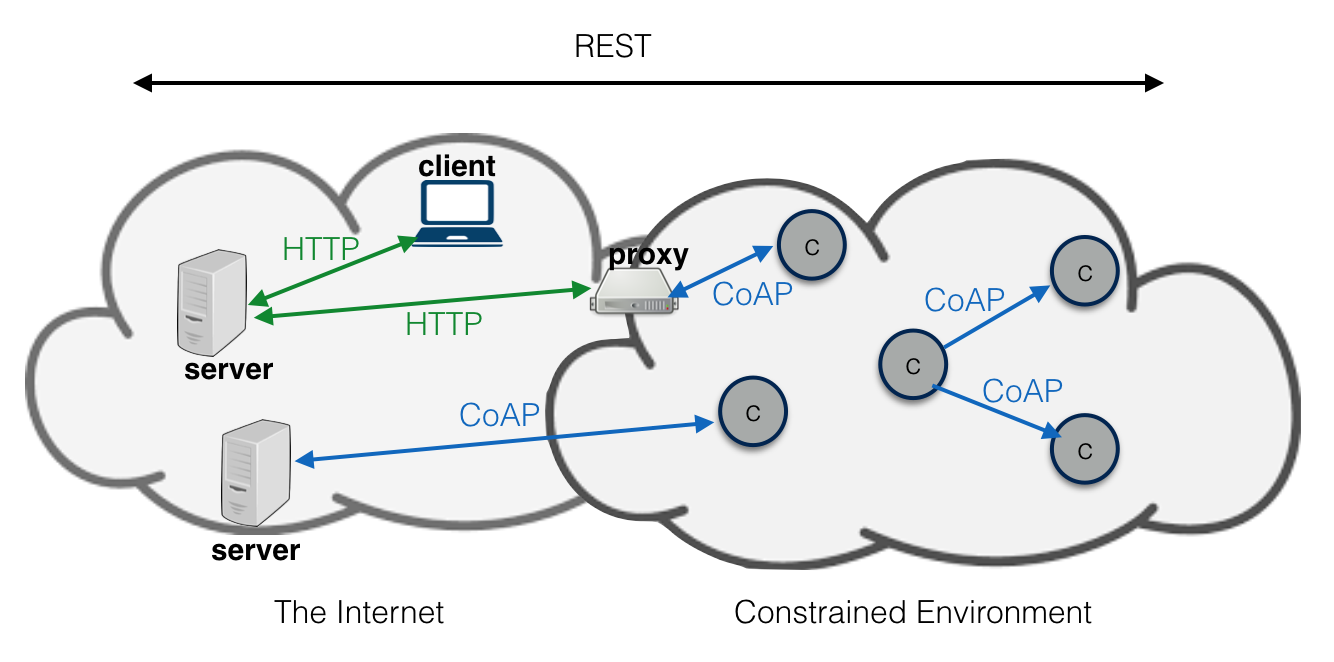
\includegraphics[scale = 0.55]{coap_app_architecture.png}
\caption{An application architecture combining CoAP and HTTP}
\label{fig:coap_app_architecture}
\end{figure}

However, CoAP is not merely a compressed version of HTTP \autocite{6159216}. It supports group communication through IP multicast. CoAP enabled devices can discover services exposed by each other via standardized interface and resource description based on the well-known resource path and Web Linking  \autocite{well_known_pattern, web_link, core_link}. CoAP allows observable resources which pushes state updates to registered clients through continuous notifications in an asynchronous manner \autocite{coap_observe}. Resource with a large body that exceeds the maximum transmission unit (MTU) can be processed using block-wise transfer, which is essentially an application layer fragmentation mechanism \autocite{blockwise}. Furthermore, alternative transports such as Short Message Service (SMS) is also feasible and is under active standardization development \autocite{coap_alter_trans}.

%it is primarily based on patterns from the Web: a client/server interaction model between application endpoints, resources that are addressable by Uniform Resource Identifiers (URIs), stateless exchange of representations that decouple client and server, uniform interfaces with standardized Internet Media Types for wide interoperability, and caching and proxying to enable high scalability \autocite{kovatsch2015scalable}.

\subsection{Comparison}


%However, CoAP seems to have a wider acceptance for constrained devices due to ease of integration with 6LowP AN, easy portability with HTTP , UDP based operation with low connection overhead, support for several features like sleeping nodes [3] (without requiring persistent connection), support for both request-response and resource- observe mode, etc.

%Comparing CoAP with MQTT, CoAP seems to have a wider acceptance for constrained devices due to the following facts: ease of integration with 6LowPAN, easy portability with HTTP, UDP based operation with low connection overhead, support for several features like sleeping nodes \autocite{coap_protocol}(without requiring persistent connection), support for both request-response and resource-observe mode. On the other hand, MQTT is ideal for integration with existing Cloud services since TCP is deployed in most infrastructures. 


MQTT is a message-oriented protocol which means that it is content agnostic and only focuses on the delivery of messages, while CoAP is all about operations against the representation of resource since it follows the REST style. Therefore, although from the perspective of implementation cost, CoAP has a wider acceptance for constrained devices due to its low overhead and better support for 6LowPAN, for less constrained devices that could afford TCP stack, MQTT is simpler to implement on the device side in terms of semantics. In addition, \textcite{6918928} pointed out other disadafvantages of resource-oriented IoT protocols like CoAP, including overhead introduced to constrained devices in terms of concurrency, computing and networking, inflexibility that IP address of each device must be known, as well as Network Address Translation (NAT) issue for global accessibility is currently most common IPv4 subnet environment. 

On the other hand, CoAP has a clear read/write semantics, which makes it not only easier to integrate with other Web-like services, but also possible to add infrastructure support for caching and proxying. MQTT's publish/subscribe architecture results in a non-intuitive way of communication when the subscriber also needs to send feedback of configuration command to the publisher since it is not the default message flow direction. Moreover, MQTT and CoAP differ a lot in terms of discovering services. With MQTT, it is necessary to first find the central server (broker) which all messages must go through. In contrast, CoAP can avoid the need for a central endpoint since it supports multicast to discover available services. The read/write semantics of CoAP then ensures independent communication endpoint to endpoint. As a result of the aforementioned difference, it requires less effort to scale CoAP than MQTT. Similarly, \textcite{kovatsch2015scalable} wrote that the main drawback of MQTT is lack of extensibility, as MQTT clients have to be pre-configured with a dedicated service similar to HTTP clients for the IoT, which makes it difficult to adapt to an evolving environment.

It should be noted that resource observation in CoAP is similar to publish/subscribe pattern in MQTT at first glance, but unlike publish/subscribe, where the goal is to propagate every event, observe only guarantees that eventually, all registered observers will have a current representation of the latest resource state. 

There are few research publications as well as industry deployments about DDS, which implies it may be still in exploration and optimization stage. On the other hand, there are known scalability \autocite{esposito2011data} and performance \autocite{sanchez2011bloom} issues associated with RTPS, which is the wire protocol used in DDS. Also, DDS's Global Data Space (GDS) concept is of limited use when faced with unreliable, low bandwidth and high latency networks \autocite{7396558}. 

\begin{table}[!htbp]
\newcolumntype{Y}{>{\centering\arraybackslash}X}
\begin{tabularx}{\textwidth}{l|c|c|c|c|c|c|c|Y}
%
			& Transport 			& RESTful 	& \makecell{Publish/\\Subscribe} 	& \makecell{Request/\\Response} 	& \makecell{Central\\Broker} 	& \makecell{Header\\Size\\(bytes)} 	& Security & Reliability \\ \hline
MQTT 		& TCP 				& \XSolid 		& \Checkmark 					& \XSolid 						& \Checkmark 				& 2 & SSL & 3 QoS levels \\ \hline
DDS 		& \makecell{TCP\\UDP} 	& \XSolid 		& \Checkmark 					& \XSolid 						& \XSolid 					& - & \makecell{SSL\\DTLS} & 23 QoS policies \\ \hline
CoAP 		& UDP 				& \Checkmark 	& \Checkmark					& \Checkmark 					& \XSolid 					& 4 & DTLS &  Stop-and-wait retransmission with exponential back-off  \\  \hline
HTTP 		& TCP 				& \Checkmark 	& \XSolid 						& \Checkmark 					& \XSolid					&  - 	& SSL & - \\ 
\end{tabularx}
\caption{A brief comparison between MQTT, DDS and CoAP}
\label{tab:mqtt_dds_coap}
\end{table}

\begin{table}[!htbp]
\centering
\begin{tabular}{l|p{5.8in}}
%\hline
%
& \multicolumn{1}{c}{Typical application} \\ \hline
MQTT & MQTT is for applications which require real-time messaging, fall into the topic-based publish/subscribe pattern and accept persistent connections to message broker. The message broker is responsible for bridging end devices to the rest of the Web. \\ \hline
DDS & DDS is for applications and system-of-systems using publish/subscribe that have to support dynamically changing environments and configurations, be constantly available, and be instantly responsive. Integrating data across many platforms and disparate systems are also necessary. \\ \hline
CoAP & CoAP is for applications that consist of constrained devices but need to run RESTful Web services to achieve direct connectivity to the Web with HTTP like methods and URIs. Usually, applications require both request/response and publish/subscribe-like interactions. \\
\end{tabular}
\caption{Potential usage of MQTT, DDS and CoAP}
\label{tab:mqtt_coap_dds_app}
\end{table}

\autoref{tab:mqtt_dds_coap} provides a brief comparison between MQTT, DDS, CoAP and HTTP in terms of architecture and semantics. HTTP is also included here as a contrast to CoAP since they share many similarities. \autoref{tab:mqtt_coap_dds_app} shows the potential application areas of the three protocols.

The resource-oriented pattern, in general, provides a more intuitive abstraction when linking devices to the Internet. The Web is a loosely-coupled application layer architecture \autocite{6159216} and so is the IoT. With such a pattern, devices connected to the Internet are viewed as unique resources (identified by URIs) and accessed through well-known methods (such as GET, PUT, POST, and DELETE) with a clear semantics about read/write and representation state (controlled by Internet Media Types). An interesting aspect of the resource-oriented pattern is that it adapts to the model of Fog Computing well. It is straightforward to model Fog as a resource or collection of resources each capable of performing basic processing tasks, which further distributes the processing load and network traffic on backend services. 

There is no IoT application layer protocol that fits all situations. As \textcite{7123563} pointed out, gateways that could interoperate with many different IoT protocols are under active research so that protocols can be deployed with much more flexibility. Among the three protocols that have been discussed, for example, MQTT could be suitable for situations where data need to be directly and reliably transferred to a server hosted on Cloud platform, while CoAP provides better support for device-to-device and device-to-Web communication. On the other hand, DDS makes more sense when deploying large-scale applications with strict real-time and QoS requirements under a reliable network environment. In the scope of this work, since the semantics of CoAP ensures its position in both Fog and Cloud, it is more straightforward to select this protocol to investigate the scalability of the IoT.

\section{CoAP Fundamentals and Implementations} \label{CoAP_intro}

This section gives an inspection of some key features and concerns of CoAP, which further shows an insight into the ideas and trade-offs made in the proposed architecture that are discussed in the following chapters. It is followed by a brief analysis of available implementations which also shows the position of this work. 

In detail, target environment of CoAP is stated in \autoref{CORE_env}; basic semantics of the core protocol is introduced in \autoref{core_protocol}; important extensions of the core protocol - resource observation and block-wise transfer are discussed in \autoref{observe_resource} and \autoref{blockwise_transfer} respectively; security issue is covered in \autoref{security}; a summary of current implementations is in \autoref{CoAP_imp}.

\subsection{Constrained RESTful Environments} \label{CORE_env}

To help the standardization work for constrained IP networks that are found in the IoT, the working group for Constrained RESTful Environments (CoRE) classifies resource-constrained devices to the following 3 classes based on their capabilities \autocite{constarined_env}: 

\begin{itemize}

\item \textbf{Class 0} devices are the most constrained ones in terms of memory and processing capabilities. Their memory sizes are x in the order of hundreds of bytes only. It is unlikely for Class 0 devices to directly communicate with the Internet securely. Usually, they rely on larger devices that behave as application-level gateways to connect to general IP based systems. 

\item \textbf{Class 1} devices are the ones with lowest capacities to directly connect to the Internet in a secure manner, which in general have about 100 KB of ROM and about 10 KB of RAM installed. Class 1 devices are not powerful enough to talk to other nodes using protocol stacks like HTTP and Transport Layer Security (TLS) but are fully capable of utilizing lightweight ones such as CoAP. 

\item \textbf{Class 2} devices are less constrained and almost capable of supporting network stacks used by smartphones or laptops, which is enabled by about 250 KB of ROM and about 50 KB of RAM. Class 2 devices can still benefit from lightweight and energy-efficient protocols so that more resources are left for applications and overall operational costs can be reduced. 

\end{itemize}

Constrained devices that are more powerful than Class 2 devices may still have some limitations, for example, they might depend on limited energy supply. Though the focus of the Constrained RESTful Environments (CoRE) working group is primarily class 1 devices, using lightweight protocols on class 2 devices and beyond enable direct interoperability between the most constrained devices and general Internet endpoints, which is essential to the IoT.

According to the above definitions, sensors and actuators are more likely to be class 0 devices. Some System on Chip (SoC) platforms fall into class 1 and may operate on behalf of the class 0 devices and expose their resources to the outside world. Other embedded platforms such as the mobile phone and the Raspberry Pi \autocite{raspberry_pi} can be seen as class 2 or beyond. They could thus perform more complex tasks and make real-time decisions based on information provided by potentially many class 0 and class 1 devices. Such a hierarchical structure naturally fits into the definition of a Fog. On the other hand, Erlang was initially deployed on telecom switches which are also embedded platforms. Therefore choosing the Raspberry Pi as the \textit{scale down} option for investigating the Erlang-based solution should be a valid match.

\subsection{Core Protocol} \label{core_protocol}

CoAP is designed to use minimal resources for both device and network. Instead of a complex transport stack, it gets by with UDP on IP. A 4-byte fixed header and a compact encoding of options enable small messages that cause no or little fragmentation on the link layer. \autoref{fig:msg_format} shows the structure of a CoAP message, which includes the four-byte base header, the variable-length token, multiple header options, and a payload carrying a representation of the resource.

\begin{figure}[!htbp]
\centering
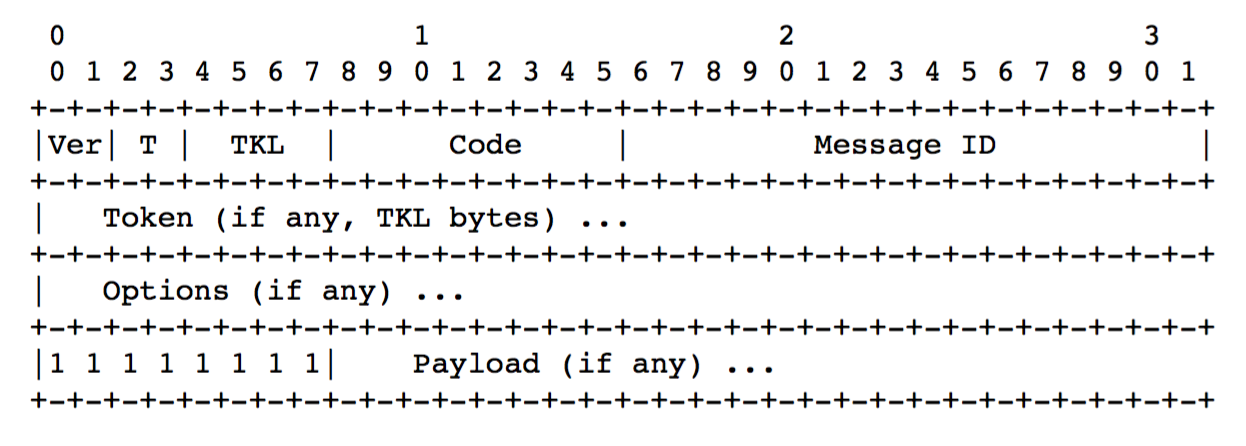
\includegraphics[scale = 0.55]{msg_format.png}
\caption[CoAP message format]{CoAP message format \autocite{coap_protocol}: A 4-byte base header containing 2 bits for versioning, 2 bits for message type encoding, 4 bits for the token length, 1 byte for the message code (either a RESTful method or a response code), and 2 bytes for the message identifier (MID), followed by a token, options and a payload.}
\label{fig:msg_format}
\end{figure}

An entity participating in the CoAP protocol is called an endpoint \autocite{coap_protocol}. It lives on a network node and is identified by its IP address, port, and security association. One can think CoAP of as having two sublayers: the request/response layer and the message layer, as shown in \autoref{fig:coap_layer}. The former handles REST communications while the latter provides duplicate detection and optional reliable delivery of messages. 

%The optional transport reliability is designed considering the characteristics of UDP and is realized using a simple stop-and-wait retransmission with exponential backoff.  


\begin{figure}[!htbp]
\centering
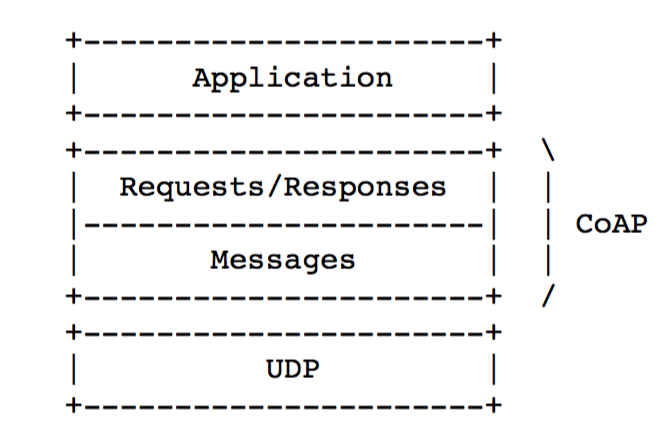
\includegraphics[scale = 0.55]{coap_layer.png}
\caption[Abstract layering of CoAP]{Abstract layering of CoAP \autocite{coap_protocol}: Request/response layer for RESTful interactions and message layer for deduplication and optional reliable delivery.}
\label{fig:coap_layer}
\end{figure}



On the message layer, messages can either be confirmable (CON), non-confirmable (NON), acknowledgements (ACK) or resets (RST). A message is identified by its message identifier (MID). CON and NON messages carry requests or responses. CON messages are used for reliable transmission. An endpoint retransmits a CON message with an exponentially increasing back-off timer until it is properly acknowledged or the maximum retransmission count is reached (which is typically 4). The response to a CON request can be sent with ACK with the same MID for message correlation (a piggybacked response), or in a separate CON response, which carries a different MID generated by the server. The separate response is useful to avoid waiting on the client side when the server can not respond instantly and can be closed by responding with an empty ACK that only contains the 4-byte base header. On the other hand, NON messages use a best-effort strategy and are not retransmitted in case of loss. A NON message can be answered with another NON message with a new MID generated by the sender. If an endpoint receives a CON or NON that it does not know how to process, it rejects it with an RST. An RST message also carries the same MID as the origin message similar to ACK, indicates failure of the message exchange and closes corresponding reliable transmission, if any. Examples of reliable and unreliable messages are shown in \autoref{fig:reliable_msg_trans} and \autoref{fig:unreliable_msg_trans} respectively.

An endpoint needs to temporarily remember incoming MIDs to detect duplicates, which are usually caused by loss of ACK messages that should close corresponding CON messages, or by network jitters. The MID of each CON and NON message should be unique in the scope of the source endpoint, and should not be reused within the lifetime of the message, which is 247 seconds for CON message and 147 seconds for NON message.  


%When an endpoint receives a confirmable message, it replies with an acknowledgement. The response to a confirmable request can be sent with the ACK, which is also called a piggybacked response, or in a separate confirmable response. The separate response is useful  to avoid waiting on client side when the server can not respond instantly. An endpoint retransmits confirmable messages with an exponentially increasing back-off timer until it receives an acknowledgement, a reset or the maximum retransmission count is reached (which is typically 4). If an endpoint receives a CON or NON that it does not know how to process, it rejects it with a RST. 


\begin{figure}[!htbp]
\begin{subfigure}[t]{.5\textwidth}
  \centering
  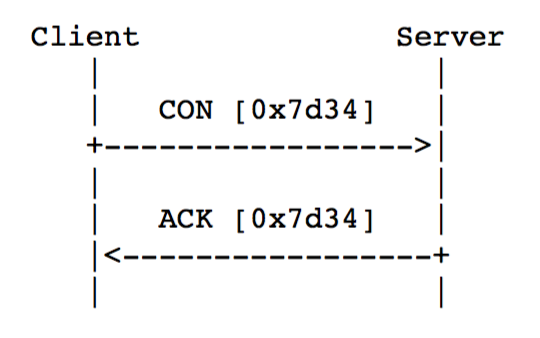
\includegraphics[scale = 0.55]{reliable_msg_trans.png}
  \caption{Reliable}
  \label{fig:reliable_msg_trans}
\end{subfigure}%
\begin{subfigure}[t]{.5\textwidth}
  \centering
  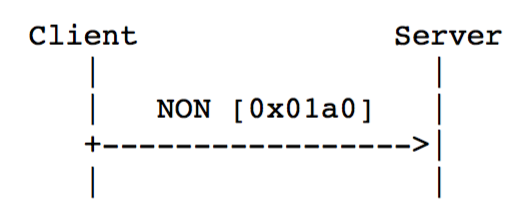
\includegraphics[scale = 0.55]{unreliable_msg_trans.png}
  \caption{Unreliable}
  \label{fig:unreliable_msg_trans}
\end{subfigure}
\caption{Example of reliable and unreliable message transmission \autocite{coap_protocol}}
\end{figure}

\begin{figure}[!htbp]
\centering
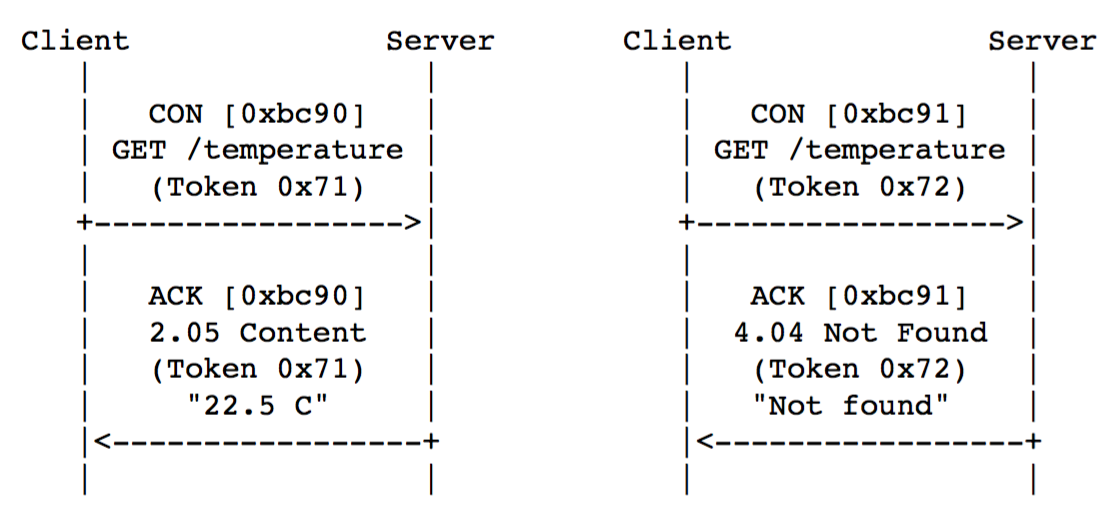
\includegraphics[scale = 0.55]{get_example.png}
\caption{Example of two GET requests with piggybacked responses \autocite{coap_protocol}}
\label{fig:get_example}
\end{figure}

On the request/response layer, requests have a method code (GET, POST, PUT, or DELETE) and responses have a response code (either of class 2.xx (success), 4.xx (client error), or 5.xx (server error)). A token (up to 8 bytes), chosen by the client, serves as the identifier for a request. The server endpoint must include the request token in the response so that the client endpoint knows to which request the response belongs to. The token must be unique at least within the scope of each destination. Additionally, CoAP requests and responses can be accompanied by simple options, similar to HTTP header options. For example, options may describe the content format or destination URI. Two examples for a basic GET request with piggybacked response are shown in \autoref{fig:get_example}, one successful, one resulting in a 4.04 (Not Found) response.

\subsection{Observing Resources} \label{observe_resource}

An essential feature for the IoT is the ability to track state change of particular data. Based on the observer pattern, the observe extension of CoAP \autocite{coap_observe} enables efficient server push notifications. It is designed as an optional feature on top of GET with an elective \verb|Observe| option. The client sets the option to zero indicating its interest in observing particular resource. If a server does not support this extension, it responds as answering a normal GET request and the client will be aware of this situation and can further attempt to repeat request for polling. When the server supports this feature, it will include this option in the response, turning it into a notification. The server tries its best to keep the interested client on its observers list as long as possible. Whenever the observed resource undergoes a change, new representations will be pushed. All notifications are subsequent responses of the original request, correlated via the request token. The \verb|Observe| option in notifications additionally provides a sequence number for reordering detection so that the client can ensure it treats the most recent notification as the freshest one. Cache control is also enabled for notifications in terms of valid lifetime, defined by the \verb|Max-Age| option. As a result, notifications are cacheable and the server would normally send a new representation before \verb|Max-Age| expires. The client would assume it is removed from the server's observer list when a representation gets stale, which may be due to an expected reboot, for instance. The client has the chance to re-register itself by sending a new observe request with the same token. It is required that all options should be identical to the original observe registration, in order for the request to match all cache keys in case any intermediary is involved. See an example of observing in \autoref{fig:coap_observe}.

\begin{figure}[!htbp]
\centering
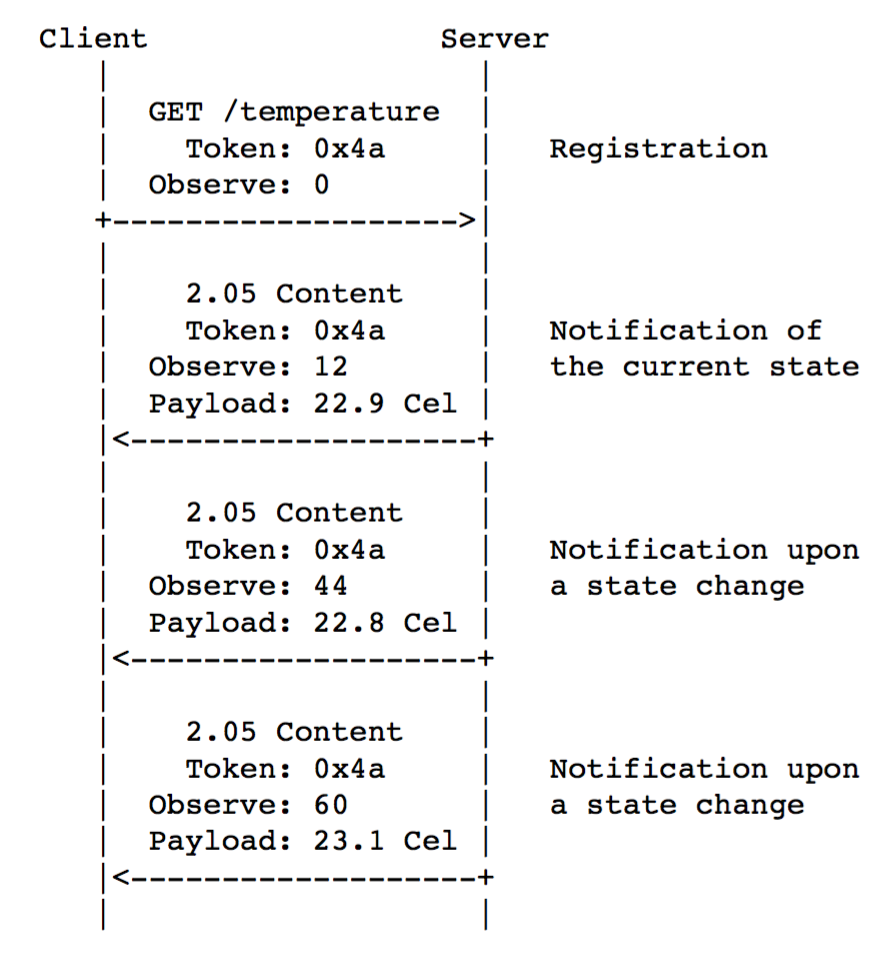
\includegraphics[scale = 0.55]{coap_observe.png}
\caption[CoAP observe synchronization]{CoAP observe synchronizes the local state with the resource state at the origin server by sending push notifications. \autocite{coap_observe}}
\label{fig:coap_observe}
\end{figure}

There are two methods to end an observe relationship once the client is no longer interested: \autocite{kovatsch2015scalable}:

\begin{itemize}

\item \textbf{Re-active cancellation:} Observers simply get rid of the local relationship states. As a result, when the next notification arrives, the client does not recognize the token and will reject it. As according to the specification the server must use a CON notification occasionally in order to detect inactive observe relations, it will eventually receive an RST which triggers the server to remove the client from its observers list. The same applies to the case where a client shuts down, making a CON notification times out.

\item \textbf{Pro-active cancellation:} If it is desired to cancel the observation in a more eager manner to save resources, clients can send a request indicating the cancellation by setting the \verb|Observe| option to one and using the token associated with the observation.

\end{itemize}

\subsection{Block-wise Transfer} \label{blockwise_transfer}

CoAP is initially designed for small payloads, which is expected from most sensor-like devices. However, sometimes applications need to transfer larger payloads, for example, updating the firmware on the fly and transferring a CoRE Link Format of resource descriptions \autocite{core_link}. Though the underlying IP layer already provides a fragmentation mechanism, it is not always feasible. CoAP uses block-wise transfer \autocite{blockwise} for these purposes. It is enabled by adding a pair of \verb|Block| options so that transferring a large resource representation can be turned into multiple request-response pairs. In detail, the \verb|Block1| option is used for uploading (PUT/POST) and the \verb|Block2| option is used for downloading (GET). Multiple block size choices are available for different scenarios. Block-wise transfer can be implemented in transparent, atomic fashion, where the application logic will only handle the complete representation after all blocks are transferred. If not, applications have to process block logic explicitly, which is beneficial for devices with limited memory as they can do this step by step.
 
 It is to be noted that block-wise transfer combined with observation will lead to only the first block to be sent as notification \autocite{blockwise}. Rest blocks need to be fetched by the client using normal GET requests. As a result, complexity on the server side is largely reduced.

\subsection{Security}\label{security}

Since Transport Layer Security (TLS) is not available for UDP, CoAP relies on Datagram Transport Layer Security (DTLS)  for security \autocite{dtls1.2, coap_protocol}. The DTLS In Constrained Environments (DICE) Working Group of the Internet Engineering Task Force (IETF) works on supporting the use of DTLS in constrained environments. Various implementations exist, for instance, tinyDTLS \autocite{tinydtls} is a C implementation targeting constrained devices, and integration of DTLS into the Java CoAP implementation Californium \autocite{californium} is discussed in a master's thesis from 2012 \autocite{jucker2012securing}. It is considered that DTLS adds extra complexity and overhead and new version of the specification that aims at reducing latency has not been finalized yet \autocite{kovatsch2015scalable}. As a result, it is not a focus of this work.




%\subsection{CoAP vs. HTTP}\label{vs_HTTP}

%It is important to note that CoAP is more than just a compressed form of HTTP and moreover provides several features that are beneficial in an M2M application. Reference \autocite{lanter2013scalability} gives a comprehensive comparison between CoAP and HTTP in terms of protocol concept as well as the processes for handling requests on server side. It shows how CoAP + UDP are superior to HTTP + TCP in constrained environments. In short, the similarities and differences are,

%\begin{itemize}
%\item \textbf{Fewer messages}: A typical CoAP exchange consists of 2 messages, i.e., a request and a response. In contrast, an HTTP request first requires the client to establish a TCP connection and later terminate it. CoAP's blockwise transfer\autocite{blockwise} though, requires an acknowledgement for each block and leads to more messages and higher transfer time. But since most CoAP messages are short, this is not a big concern.

%\item \textbf{Compressed format}: CoAP encodes option values in binary format while an HTTP request is one large, verbose text. A minimum CoAP header is only 4 bytes long and a minimum UDP header is only 8 bytes long. In contrast, a minimum TCP header alone is 20 bytes long plus what comes from HTTP. A bare CoAP request is not human-readable though.

%\item \textbf{Observe pattern}: Observe pattern is basically such a process: a client declares its interest in the occurrence of a specific type of event to a server and is notified by the server when such an event occurs. In CoAP, a client can establish such an observe relation with a resource which sends a notification when its state changes. This is not available in HTTP.

%\item \textbf{Resource discovery}: CoAP defines a well-known URI \textit{/.well-known/core} which lists the URIs to available resources on a CoAP endpoint. URIs and descriptions of resources are encoded in the Core Link Format \autocite{core_link} and can be requested by a GET request from a client. This mechanism allows autonomous devices and services to efficiently discover other CoAP resources in a uniform and standardized way. While crawling achieves similar goal with HTTP, but is highly inefficient in terms of data exchange.

%\item \textbf{Group communication}: CoAP supports making requests to an IP multicast group \autocite{coap_protocol}. It allows a client to address multiple servers at once. This can obviously save some effort for the client and can especially be useful for discovery. IP multicast violates TCP's connection oriented paradigm, and is therefore not applicable for HTTP.

%\item \textbf{Deduplication}: A disadvantage of CoAP is that it has to detect and filter duplicates on its own, unlike HTTP, which inherits the reliability guarantees from TCP. A CoAP server identifies a message by the pair of its source and message identifier (MID) and has to remember it for a specific time (247 seconds for confirmable messages and 145 seconds for non-confirmable messages). This may add extra overhead in terms of memory consumption and book-keeping effort.
%\end{itemize}

%\begin{table}[!htbp]
%\centering
%\begin{tabular}{lll}
%%
% & \bfseries CoAP &  \bfseries HTTP \\ \hline
%\bfseries 1 & Get the datagram from the socket & Accept connection \\
%\bfseries 2 & Interpret the request & Interpret the request \\
%\bfseries 3 & Translate the path and find the response & Translate the path and find the requested file (location) \\
%%
%& \textbf{a)} From the cache & \textbf{a)} From the cache \\
%%
%& \textbf{b)} Search in the resource tree & \textbf{b)} Search on the disk \\
%\bfseries 4 & - & Send the response header \\
%\bfseries 5 & Handle the request and prepare a response & Read the file to the cache (if necessary) \\
%\bfseries 6 & Send the response & Send the response body \\
%\end{tabular}
%\caption{Structures of the processes for handling CoAP and HTTP requests}
%\label{tab:coap_vs_http}
%\end{table}

%And in terms of request processing, \autoref{tab:coap_vs_http} \autocite{lanter2013scalability} lists different steps that would happen when handling a request of CoAP/HTTP. Note that a traditional HTTP server is used for loading files from local disks and serving them online for clients, if the files are not dynamically generated Web pages, while a CoAP server usually holds a data structure (maybe in memory) of the resources or generates a response using other resource on the fly.  

\subsection{CoAP Implementations}\label{CoAP_imp}

Several CoAP implementations already exist and either target constrained or unconstrained platforms. 

For embedded platforms, there are a variety of optimized implementations including CoAPBlip for TinyOS \autocite{6208761}, SMCP \autocite{SMCP}, libcoap \autocite{kuladinithi2011implementation}, Erbium (Er) for Contiki \autocite{kovatsch2011low} and CoAPSharp \autocite{coapsharp} for the .NET Micro Framework. Cantcoap \autocite{cantcoap} is a CoAP implementation that focuses on simplicity by offering a minimal set of functions and a straightforward interface. Being a C implementation, however, it only focuses on decoding and encoding, leaving the actual protocol to the application. Although these implementations can also be deployed on an unconstrained platform, they are not designed for scalability and not suitable for performing complex services.

OpenWSN \autocite{open-wsn} is a comprehensive IoT project at UC Berkeley. Its main aspect is high reliability for low-power communication. Besides a full software stack for sensor nodes, OpenWSN offers a CoAP Python library \autocite{openwsn_python} to implement backend services. It primarily targets easy interaction with OpenWSN devices and is not designed for scalability.

CoAPthon \autocite{coapthon_code, 7389028} is another Python library for CoAP built on top of the Twisted framework \autocite{twisted}. It targets embedded systems or above, favouring easy development over large scalability. 

The Sensinode NanoService Platform is a commercial solution that offers good support for industry-relevant features \autocite{kovatsch2015scalable}. At the time of writing, it has become part of the ARM mbed platform \autocite{mbed} since the Sensinode start-up has been acquired by ARM at an earlier time. Java and C libraries are included for both devices and Cloud. However, these libraries are commercial and not publicly available. 

mjCoAP is a lightweight and open-source CoAP implementation written in Java which targets less constrained embedded devices such as Raspberry Pi and middle-class smartphones \autocite{cirani2015mjcoap}. Its design goals include interoperability, development simplicity, and code reusability rather than scalability.  

There are two open-source Java frameworks jCoAP \autocite{jcoap} and nCoAP \autocite{ncoap} which target unconstrained platforms. The former one only implements an early draft version of CoAP at the time of writing thus is incompatible with the current CoAP standard. While the latter one, according to \autocite{lanter2013scalability}, may still be in early optimization stage and have problems that affect its performance.

Californium (Cf) \autocite{californium} is a modular, open-source framework that facilitates deployment of backend services, serving as an intermediary between the logic of a service and the IoT. It originated from the research in ETH, Switzerland and has become an Eclipse Foundation project since 2014. With its core based in Java, it aims at providing scalable backend services for CoAP in the Cloud and has shown better performance than other implementations \autocite{lanter2013scalability, kovatsch2014californium, kovatsch2015scalable}. It also targets unconstrained platforms hence it makes more sense to run Californium on commodity server machines rather than on constrained devices, though it is still available on some embedded platforms due to Java's portability. 

\textcite{muller2015coap} explored the possibility of using common Web application frameworks for HTTP such as Ruby on Rails in the Internet of Things utilizing CoAP and proposed a CoAP server implementation in Ruby called David \autocite{david}. It puts more emphasis on interoperability between common Web applications and CoAP and to what extent existing Web framework can be reused in IoT scenarios. The architecture of David is inspired by Californium and it has a similar or less performance as Californium. 
 
Copper (Cu) \autocite{copper} is a CoAP user-agent for Firefox implemented in JavaScript. It enables users to browse IoT devices in the same fashion they are used to explore the Web. This is done by providing a presentation layer that is originally missing in the CoAP protocol suite. Its ability to render a number of different content types such as JSON or the CoRE Link Format \autocite{core_link} makes it a useful testing tool for application as well as protocol development \autocite{jucker2012securing}. Copper is meant to run only as a client.

\begin{table}[!htbp]
\centering
\begin{tabular}{l|c|c|c|c|c}
%
&
Language & CoAP Version  & Target Platform & Scalability & Fault-tolerance \\ \hline
CoAPBlip & nesC/C & CoAP-13 & Very Constrained & No & - \\ 
SMCP & C & RFC & Very Constrained & No & - \\
libcoap & C & RFC &  Very Constrained & No & - \\
Erbium & C & RFC & Very Constrained & No & - \\ 
Cantcoap & C++/C & RFC & Very Constrained & No & - \\
CoAPthon & Python & RFC & Constrained & No & - \\
CoAP/OpenWSN & Python & CoAP-18 & Unconstrained & No & - \\
CoAPSharp & C\# & RFC & Constrained & No & - \\
mjCoAP & Java & RFC & Constrained & No & - \\
jCoAP & Java & - & Unconstrained & - & - \\
nCoAP & Java & RFC & Unconstrained & Yes & - \\
Californium & Java & RFC & Unconstrained & Yes & - \\
David & Ruby & RFC & Unconstrained & Yes & - \\
Copper & JavaScript & RFC & Web Browser & - & -
\end{tabular}
\captionsetup{format=hang}
\caption[Brief summary and comparison of major CoAP implementations]{Brief summary and comparison of major CoAP implementations. Target environment ranges from very constrained to unconstrained, which covers sensors, more powerful embedded systems and Cloud backends. - implies not applicable or not mentioned clearly.}
\label{tab:coap_imp_compare}
\end{table}


A brief summary and comparison between major CoAP implementations are shown in \autoref{tab:coap_imp_compare}. Some details about certain implementations are temporarily not available at the time of writing. The column scalability/fault-tolerance means whether the implementation declares itself as designed for scalability/with fault-tolerance in mind or relevant tests show these features. Current and comprehensive lists of CoAP implementations are to be found in the Wikipedia \autocite{coap_wiki} and on the Website coap.technology \autocite{coap_tech}.

\autoref{tab:coap_imp_compare} shows that major CoAP implementations either target constrained devices with poor support for scalability, or equip with full support for scalability but target unconstrained platforms such as the Cloud. Many CoAP server implementations such as jCoAP, CoAP Python library from OpenWSN and CoAPthon use Single-Process-Event-Driven (SPED) architecture which implies lacking support for scalability when it comes to multi-core environment \autocite{kovatsch2015scalable}. On the other hand, there is a silence on fault-tolerance feature. Among these popular implementations, the lack of a combination of scalability and fault-tolerance within one solution that has a wider usage scenario ranging from less constrained embedded platform to resource-rich Cloud backend reduces flexibility for potential IoT applications.

The summary does not include information on implementations based on concurrency-oriented languages, though. By the time of writing, there is only one publicly available CoAP client/server implementation in Erlang called gen\_coap \autocite{gen_coap}, which is not under active development though. The ecoap prototype is inspired by some of its insights. The main motivation of developing another Erlang implementation is that gen\_coap is more a proof of concept and only gives a rough idea on how concurrency can be modelled in Erlang. Many designs of gen\_coap has to be reconsidered in the context of this thesis. For instance, the relationship between different components, the data flow of request handling and fault-tolerance policy. Moreover, it lacks performance evaluation both under constrained and unconstrained environment. Local tests during development show that the proposed prototype has improved performance. Despite gen\_coap, no other complete CoAP library in Erlang is publicly available. Some implementations utilizing other concurrency-oriented languages such as Go \autocite{go} exist, namely go-coap \autocite{go-coap} and canopus \autocite{canopus}. However, both projects are incomplete as they only implemented part of the whole core specification. 
 
%Different from implementations listed in table \ref{tab:coap_imp_compare}, this work aims at evaluating to what extent an implementation could both scale up (in the Cloud) and scale down (under relatively constrained environment).  Meanwhile fault-tolerance is checked through comparing performance under ordinary operation and when one or more faults are injected on purpose. As the state-of-the-art implementation which was designed with scalability in mind and has verified high performance over other implementations (as stated in \autocite{kovatsch2014californium}\autocite{kovatsch2015scalable}), Californium is selected as the performance reference during the evaluation of this work.

Few benchmark tools for CoAP server performance testing have been presented, among which, CoAPBench from Californium (Cf) Tools \autocite{coapbench} is a relatively widely adopted benchmark tool. Like Californium, it is also developed using Java. However, in order to generate high concurrent virtual clients for stress testing, the distribution mode which uses a cluster of machines to run the benchmark has to be employed. For the sake of simplicity, an Erlang benchmark tool following the same idea of CoAPBench has been developed and used for evaluation of this work. More details of the benchmark tool are discussed in \autoref{ecoap_bench}.
